\documentclass[11pt a4paper]{article}
\usepackage[greek,english]{babel}
%\usepackage[square]{natbib}
\usepackage{amsmath,amssymb,amsthm}
\usepackage{mathrsfs,bm}
\usepackage{graphicx,epstopdf,caption}
\usepackage{float,subcaption,setspace,booktabs,multirow,supertabular,lscape,threeparttable}
\usepackage{float,colortbl}
\usepackage{placeins}
\usepackage{indentfirst}
\usepackage{enumitem}
\setlength{\parindent}{0pt} %% noindent for the entire file % or add indent {2em}
\usepackage{geometry}
\geometry{left=1in,right=1in,top=1in,bottom=1in}
\usepackage[noblocks]{authblk}
\usepackage{lipsum}%% a garbage package you don't need except to create examples.
\usepackage{fancyhdr}
\pagestyle{fancy}
\rhead{You Name}  % set your name here
\lhead{Stat 8051}
\renewcommand{\headrulewidth}{0.4pt}
\usepackage[svgnames]{xcolor}
\usepackage{listings}
\usepackage{verbatim}
\lstset{language=R,
	basicstyle=\small\ttfamily,
	stringstyle=\color{DarkGreen},
	otherkeywords={0,1,2,3,4,5,6,7,8,9},
	morekeywords={TRUE,FALSE},
	deletekeywords={data,frame,length,as,character},
	keywordstyle=\color{blue},
	commentstyle=\color{DarkGreen},
}
\usepackage{Sweave}
\graphicspath{{Figures/}}  % set the path of figures
\usepackage{blindtext}
\usepackage{scrextend}
\addtokomafont{labelinglabel}{\bfseries}
\usepackage{listings}

	

\begin{document}

\title{Homework 0}
\author{My Name}  %% set your name on the main page
\date{\vspace{-5ex}}  % suppress the output of date
\maketitle

\section{Model Building}

\subsection{Data Preprocessing}

\textbf{\textit{Multicollinearity Analysis}}: Generate a correlation diagram of the covariates to investigate the relationship between variables. As shown in Figure \ref{fig:resid-m0} and Table   \ref{table:var-group}, ...


\textbf{\textit{Transformation and Residual Analysis}}: The next step is to check model assumptions and transformation.



\subsection{Model Summary}
The estimated model is shown as below. The residual standard error is 0.3 and the AIC value is -67. The detail of the summary is shown in Output 1.

\begin{equation}\nonumber
\begin{aligned}
\tilde{y} &=12 + 0.2*V5\\
&- 0.01*V15:V12 \\
y &= (75\tilde{y}+1)^{2/3}-20 \\
\end{aligned}
\end{equation}






\section{Important Variables and Reliability Assessment}
Combing the result of model comparison, the final model ...


\section{Model Comparison}
Compare the proposed model \textbf{m1} with candidate models: regression tree, random forest, bagging \cite{faraway2016extending} , ... The optimal lo and gam model are as follows:
\verbatiminput{outputs/nonparam.txt}



You can also insert your code using the following code: 

\begin{lstlisting}[language=R]
fib <- function(n) {
if (n < 2)
n
else
fib(n - 1) + fib(n - 2)
}
fib(10) # => 55
\end{lstlisting}



\subsection*{Problem 1}  %% * means no number

\textbf{(a).}
\begin{Schunk}
\begin{Sinput}
> # library(oehlert)
>   library(faraway)
>   library(MASS)
> # m<-lm(durability ~ brand, data = ex11.3)
> # boxcox(m)
> # anova(m)
> n<-6;g<-5
> l<-(80.45*qf(0.005,25,4)-1)/n;u<-(80.45*qf(0.995,25,4)-1)/n
> l;u
\end{Sinput}
\begin{Soutput}
[1] 2.606462
\end{Soutput}
\begin{Soutput}
[1] 268.0322
\end{Soutput}
\end{Schunk}
I don't believe this interval has 99\% coverage because the assumption may not satisfied. Brand 1 is very different form other brands, which means $\alpha_1$ may not follow a normal distriution.\\

\textbf{(b).}
\begin{Schunk}
\begin{Soutput}
[1] 0.7930562
\end{Soutput}
\begin{Soutput}
[1] 0.9912905
\end{Soutput}
\end{Schunk}








\nocite*{}  
%\bibliographystyle{apalike}  %disordered
%\bibliographystyle{plain}  %ordered by auther
%\bibliographystyle{unsrt}  %ordered as referenced
\bibliographystyle{IEEEtranN}
\bibliography{bibfile}


\newpage
\section*{Appendices}

\subsection*{Appendix A: Figures}

\begin{figure}[H]
	\centering
	\begin{subfigure}{.7\textwidth}
		\centering
		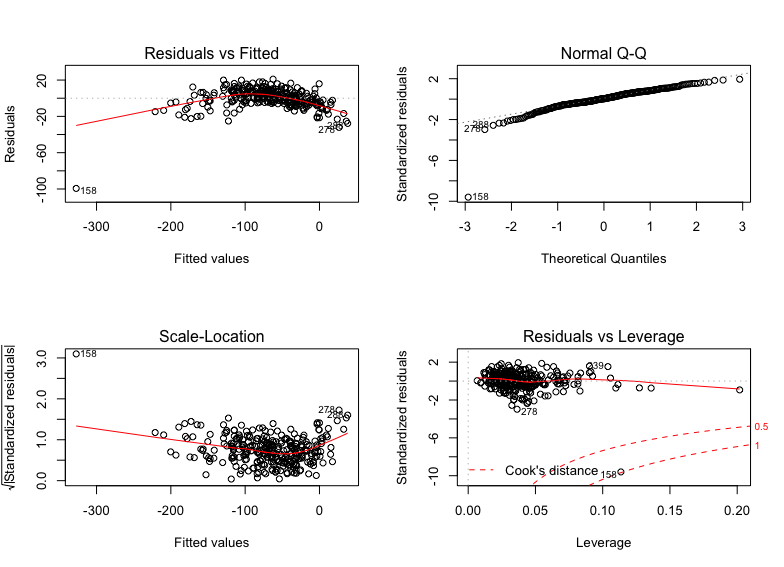
\includegraphics[scale=0.4]{resid-m0.png}
		\caption{Residual Plots of lm(y $\sim$ .)}
		\label{fig:resid-m0}
	\end{subfigure}%
	\begin{subfigure}{.3\textwidth}
		\centering
		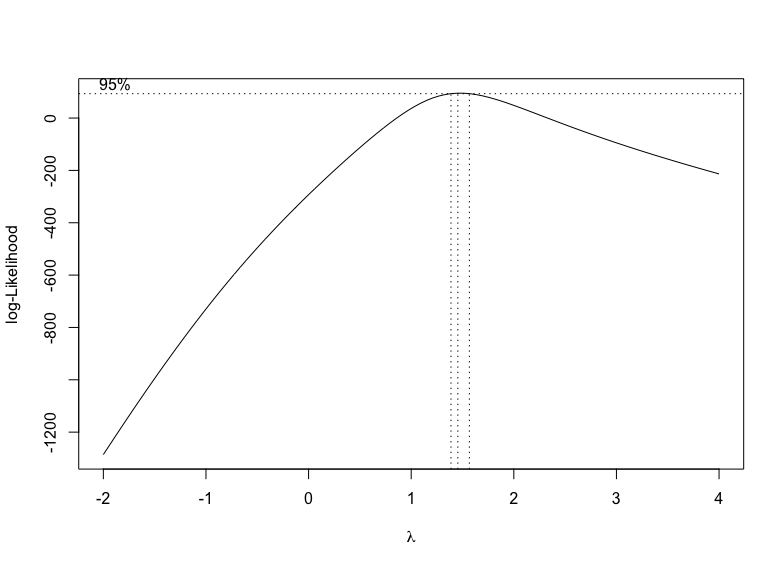
\includegraphics[scale=0.2]{boxcox-m0.png}
		\caption{BoxCox Plot of lm(y $\sim$ .)}
		\label{fig:boxcox-m0}
	\end{subfigure}
	\caption{Diagnostics Plots of lm(y $\sim$ .)}
	\label{fig:diagnostics-m0}
\end{figure}


\begin{figure}[H]
	\centering
	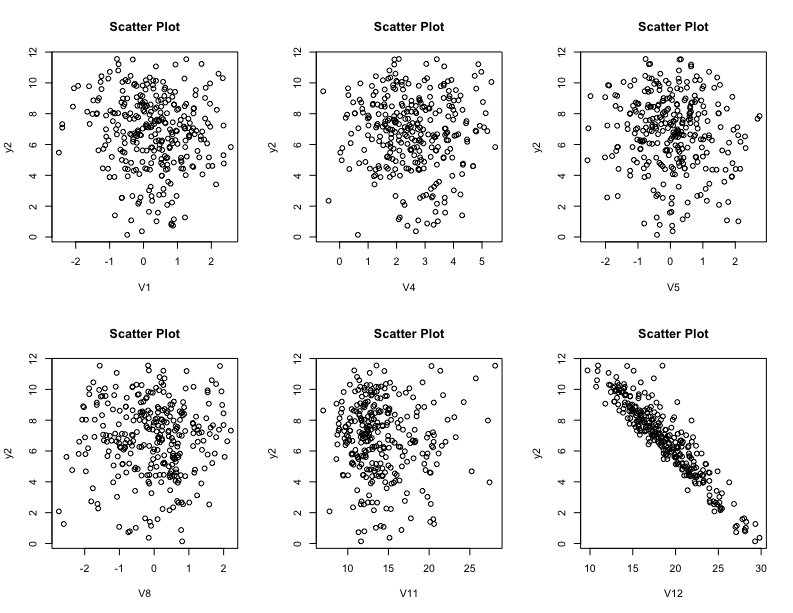
\includegraphics[scale=0.45]{scatter1.png}
	\caption{Scatter plot between response and variables}
	\label{fig:scatter1}
\end{figure}




\subsection*{Appendix B: Tables}

\begin{table}[H]
	\centering
	\caption{Grouping of Variables}
	\begin{tabular}{c|cccc}
		\hline
		$G0$ & 1 & 2 & 3 & 4  \\
		$G1$ & 5 & 6 & 7 &   \\
		\hline
	\end{tabular}
	\label{table:var-group}
\end{table}

\begin{table}[H]
	\centering
	\caption{Variables selected and VSD values}
	\begin{tabular}{c|ccccccc}
		\hline
		\multirow{2}{*}{$method$} & \multirow{2}{*}{$Variables$} & \multicolumn{3}{c}{\textsl{ARM}} & \multicolumn{3}{c}{\textsl{BIC}} \\
		\cline{3-8}
		&  & \textsl{VSD} & \textsl{VSD\_minus} & \textsl{VSD\_plus} & \textsl{VSD} & \textsl{VSD\_minus} & \textsl{VSD\_plus} \\
		\hline
		LASSO & \{1 2 3 4\} & 0 & 0 & 0  & 0 & 0 & 0  \\
		SCAD & \{1 2 3\} & 0 & 0 & 0  & 0 & 0 & 0 \\
		MCP & \{1 2\} & 0 & 0 & 0  & 0 & 0 & 0 \\
		\hline
	\end{tabular}
	\label{table:vsd}
\end{table}

\begin{table}[H]
	\centering
	\caption{Variable Importance}
	\begin{tabular}{c|c}
		\hline
		Metric & Importance Order\\
		\hline
		IncMSE & 1 2 3 4  \\
		IncNodePurity & 1 2 3 4  \\
		SOIL & 1 2 3 4  \\
		 & (leftmost is the most important) \\
		\hline
	\end{tabular}
	\label{table:var-importance}
\end{table}

\begin{table}[H]
	\centering
	\caption{Uncertainty Assessment}
	\begin{tabular}{cc|c}
		\hline
		\multicolumn{2}{c|}{\textsl{Method}}& S=\{1, 2, 3, 4\}  \\
		\hline
		\multirow{3}{*}{\textsl{Instability}} & Sequential & 0\\
		& Bootstrap & 0 \\
		& Perturbation & 0 \\
		\hline
		\multirow{5}{*}{\textsl{ARM}} & \textsl{VSD} & 0 \\ 
		& \textsl{VSD\_minus} & 0 \\
		& \textsl{VSD\_plus} & 0 \\
		& \textsl{F-measure} & 0 \\
		& \textsl{G-measure} & 0 \\
		\hline
		\multirow{5}{*}{\textsl{BIC}} & \textsl{VSD} & 0 \\ 
		& \textsl{VSD\_minus} & 0 \\
		& \textsl{VSD\_plus} & 0 \\
		& \textsl{F-measure} & 0 \\
		& \textsl{G-measure} & 0 \\
		\hline
	\end{tabular}
	\label{table:uncertainty}
\end{table}

\begin{table}[H]
	\centering
	\caption{Model Comparison}
	\begin{tabular}{l|cc}
		\hline
		Comparison & Winner & Winning Fraction of m1\\
		\hline
		m1 vs. Regression Tree & m1 & 1 \\
		m1 vs. random forest & m1 & 1 \\
		m1 vs. bagging & m1 & 1 \\
		m1 vs. loess & m1 & 1 \\
		m1 vs. gam & gam & 0 \\
		\hline
	\end{tabular}
	\label{table:compare}
\end{table}

\begin{table}[H]
	\centering
	\caption{Cross Validation MSE and Absolute Error}
	\begin{tabular}{l|cc}
		\hline
		Model & CV MSE & CV Mean Absolute Error\\
		\hline
		m1 				& 0	& 0 \\
		Regression Tree & 0	& 0 \\
		random forest 	& 0	& 0 \\
		bagging 		& 0	& 0 \\
		loess 			& 0	& 0 \\
		gam 			& 0	& 0 \\
		\hline
	\end{tabular}
	\label{table:mse}
\end{table}


%  \newpage   % to set a new page

\subsection*{Appendix C: R output}
\noindent\textbf{Output 1}
\verbatiminput{outputs/mod-summary.txt}







\end{document}